\documentclass[12pt,a4paper]{article}
\usepackage[utf8]{inputenc} % sempre salve seus arquivos como UTF8
\usepackage[T1]{fontenc}
\usepackage[brazil]{babel}

\usepackage[left=2.5cm,right=2cm,top=2cm,bottom=2.5cm]{geometry}
\usepackage{amsmath}
\usepackage{amsthm}
\usepackage{amsfonts}
\usepackage{graphicx}
\usepackage{algorithm}
\usepackage{color}
\usepackage[noend]{algpseudocode}
\usepackage{mathtools}

% load times font
\usepackage{mathptmx}
\usepackage[scaled=.90]{helvet}
\usepackage{courier}

% comandos
\newcommand{\mdc}[1]{\mathrm{mdc}(#1)}

\DeclarePairedDelimiter\ceil{\lceil}{\rceil}
\DeclarePairedDelimiter\floor{\lfloor}{\rfloor}


\definecolor{mygray}{gray}{0.4}

\title{MO446 -- Introduction to Computer Vision  \\ Project 0}
\author{Breno Leite  \\ Guilherme Leite}
\date{10/08/2017}

\begin{document}

\maketitle

\begin{enumerate}
\item
\item
\begin{enumerate}
\item The operation was made by switching the two components (Red and Blue) of the image, since the colored image has three components (Red, Green and Blue) the Green one was left untouched and the two remaining were switched between themselves, resulting in image \ref{p0-2-a-0}.

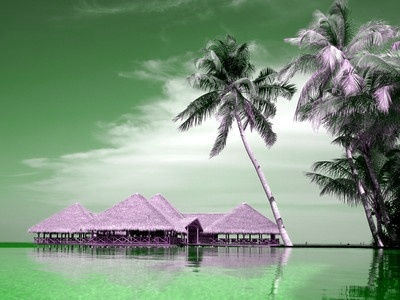
\includegraphics[]{p0-2-a-0}

\item Monochrome images are composed only with shades of gray, represented in a discrete matrix of values between 0 to 255, in the other hand colored images are represents by three components which also range from 0 to 255 each. It was possible to create a monochrome image by using the value of the green channel alone and ignoring the other two, resulting in image IMAGE\_NUMBER.

\item The same as above was done here, now using only the red value of the image, resulting in image IMAGE\_NUMBER.

\item The image made from the green channel looks more like what we expected, probably because of our nature sensibility to the green color, hence using it to create a image looks more aligned with what a human would expect.
\end{enumerate}

\item
\begin{enumerate}
\item .

\item .
\end{enumerate}

\item
\begin{enumerate}
\item .

\item .

\item .
\end{enumerate}

\item
\begin{enumerate}
\item .

\item .

\item .
\end{enumerate}

\end{enumerate}
\end{document}
